\section{MAB Formulation for Deformable Object Manipulation}

% \begin{wrapfigure}[20]{r}{0.6\textwidth}
    % \vspace{-0.62in}
    % \begin{minipage}{0.6\textwidth}
        \begin{algorithm}[t]
            \caption{MainLoop$(\obstacle, \beta, \lambda)$}
            \begin{algorithmic}[1]
                \State $t \gets 0$
                \State $\relaxeddistancematrix \gets$ GeodesicDistanceMatrix$(\deformconfig_{relaxed})$
                \State $\modelset \gets$ InitializeModels$(\relaxeddistancematrix)$
                \State InitialzeBanditAlgorithm()
                \State $\deformconfig(0) \gets$ SensePoints()
                \State $\robotconfig(0) \gets$ SenseRobotConfig()
                \While{true}
                    \State $\modelchosen \gets $ SelectArmUsingBanditAlgorithm()
                    
                    \State $\deformtarget \gets$ GetTargets()
                    \State $\deformvelocity_e, \pseudoinverseweight_e \gets$ ErrorCorrection$(\deformconfig(t), \deformtarget)$
                    \State $\deformvelocity_s, \pseudoinverseweight_s \gets$ StretchingCorrection$(\relaxeddistancematrix, \lambda, \deformconfig(t))$
                    \State $\deformvelocity_d, \pseudoinverseweight_d \gets$ CombineTerms$(\deformvelocity_e, \pseudoinverseweight_e, \deformvelocity_s, \pseudoinverseweight_s)$
        
                    \State $\robotvelocity_d \gets \deformablemodelbackwardfunction_m(\deformvelocity_d, \pseudoinverseweight_d)$
                    \State $\robotvelocity \gets$ ObstacleRepulsion$(\robotvelocity_d, \obstacle, \beta)$
                    \State CommandConfiguration$(\robotconfig(t) + \robotvelocity)$
        
                    \State $\deformconfig(t + 1) \gets$ SensePoints$()$
                    \State $\robotconfig(t + 1) \gets$ SenseRobotConfig$()$
                    \State UpdateBanditAlgorithm$()$
                    
                    \State $t \gets t + 1$
                \EndWhile
            \end{algorithmic}
            \label{alg:mainloop}
        \end{algorithm}
    % \end{minipage}
% \end{wrapfigure}

\begin{figure}[ht]
    \centering
    \includegraphics[height=1.5in]{EuclideanVsGeodesic}
    \caption{Euclidean distance measures length of the shortest path between $p_i$ and $p_j$ in $\reals^3$ (gold). Geodesic distance measures the length of the shortest path, constrained to stay within the deformable object (red).}
    \label{fig:distance}
\end{figure}

Our algorithm~(Alg.~\ref{alg:mainloop}) can be broken down into four major sections and an initialization block. In the initialization block we pre-compute the geodesic distance (see Fig.~\ref{fig:distance}) between every pair of points in $\deformconfig$ when the deformable object is in its ``natural'' or ``relaxed'' state and store the result in $\relaxeddistancematrix$. These distances are used to construct the deformation models~(Sec.~\ref{sec:jacobian_models}), as well as to avoid overstretching the object~(Sec.~\ref{sec:desired_direction}).
At each iteration we: 
1) pick a model to use to achieve the desired direction~(Sec.~\ref{sec:bandit_algorithms}); 
2) compute the task-defined desired direction to move the deformable object~(Sec.~\ref{sec:desired_direction}); 
3) generate a velocity command using the chosen model~(Sec.~\ref{sec:jacobian_models}); 
4) modify the command to avoid obstacles~(Sec.~\ref{sec:desired_direction});
and 5) update bandit algorithm parameters~(Sec.~\ref{sec:bandit_algorithms}).


\subsection{Algorithms for MAB}
\label{sec:bandit_algorithms}

Previous solutions~\cite{Auer2002,Granmo2010} to minimizing~\eqref{eqn:totalregret} assume that rewards for each arm are normally and independently distributed and then estimate the mean and variance of each Gaussian distribution.  We test three algorithms in our experiments: Upper Confidence Bound for normally distributed bandits UCB1-Normal, Kalman Filter Based Solution to Non-Stationary Multi-arm Normal Bandits (KF-MANB), and our extension of KF-MANB, Kalman Filter Based Solution to Non-Stationary Multi-arm Normal Dependent Bandit (KF-MANDB).



\subsubsection{UCB1-Normal}
The UCB1-Normal algorithm~\cite{Auer2002} (Alg.~\ref{alg:ucb1normal}) treats each arm (model) as independent, estimating an optimistic Upper Confidence Bound (UCB) for the utility of each model. The model with the highest UCB is used to command the robot at each timestep. This algorithm assumes that the utility of each model is stationary, gradually shifting from exploration to exploitation as more information is gained. While our problem is non-stationary and dependant, we use UCB1-Normal as a baseline algorithm to compare against due to its prevalence in previous work.

\begin{algorithm}[t]
    \caption{UCB1-Normal - reproduced from~\cite{Auer2002}}
    \label{alg:ucb1normal}
    \begin{algorithmic}
        \For{$t = 1,2,\dots$}
            \vspace{-11pt}
            \State{
                \begin{itemize}
                    \item If there is an arm which has been pulled less than $\ceil*{8 \log t}$ times then pull this arm. If multiple arms qualify, we select the arm that has been pulled less, selecting the arm with the lower index in the case of a tie.
                    \item Otherwise pull arm $j$ that maximizes
                        \begin{equation*}
                            \bar \utility_j + \sqrt{16 \cdot \frac{q_j -n_j \bar \utility_j^2}{n_j - 1} \cdot \frac{\ln(t-1)}{n_j}}
                        \end{equation*}
                        where $\bar \utility_j$ is the average reward obtained from arm~$j$, $q_j$ is the sum of squared rewards obtained from arm~$j$, and $n_j$ is the number of times arm~$j$ has been pulled so far.
                    \item Update $\bar \utility_j$ and $q_j$ with the obtained reward $r_j$.
                \end{itemize}
            }
        \EndFor
    \end{algorithmic}
\end{algorithm}


\subsubsection{KF-MANB}
The Kalman Filter Based Solution to Non-Stationary Multi-arm Bandit (KF-MANB) algorithm~\cite{Granmo2010} (Alg.~\ref{alg:kf-manb}) uses independent Kalman filters to estimate the utility distribution of each model, and then uses Thompson sampling~\cite{Agrawal2012} to chose which model to use at each timestep. Because this algorithm explicitly allows for non-stationary reward distributions, it is able to ``switch'' between models much faster than UCB1-Normal.

\renewcommand{\algorithmicrequire}{\textbf{Input:}}
\renewcommand{\algorithmicensure}{\textbf{Initialization:}}
\begin{algorithm}[t]
    \caption{KF-MANB - reproduced from~\cite{Granmo2010}}
    \label{alg:kf-manb}
    \begin{algorithmic}
        \Require Number of bandit arms $\nummodels$; Observation noise $\observationnoisefactor^2$; Transition noise $\transitionnoisefactor^2 \utilityprocessscale^2$.
        \Ensure $\bar \utility_1(1) = \bar \utility_2(1) = \dots = \bar \utility_\nummodels(1) = A$; $\sigma_1(1) = \sigma_2(1) = \dots = \sigma_\nummodels(1) = B$; \textit{\# Typically, $A$ can be set to $0$, with $B$ being sufficiently large}
        \For{$t = 1,2,\dots$}
            \vspace{-11pt}
            \State{
                \begin{enumerate}
                    \item{For each arm $j \in \{1,\dots,\nummodels\}$}, draw a value $x_j$ randomly from the associated \textit{normal} distribution $f(x_j;\bar \utility_j(t),\sigma_j(t))$ with the parameters $(\bar \utility_j(t),\sigma_j(t))$.
                    \item{Pull the arm $i$ whose drawn $x_i$ is the largest one:
                        \begin{equation*}
                            i = \argmax_{j \in \{1,\dots,\nummodels\}} x_j.
                        \end{equation*}
                    }
                    \item{Receive reward $\tilde r_i$ from pulling arm $i$, and update parameters as follows:
                        \begin{itemize}
                            \item{Arm $i$:
                                \begin{align*}
                                    \bar \utility_i(t+1)      &= \frac{(\sigma_i^2(t) + \transitionnoisefactor^2 \utilityprocessscale^2) \cdot \tilde r_i + \observationnoisefactor^2 \cdot \bar \utility_i(t)}{\sigma_i^2(t) + \transitionnoisefactor^2 \utilityprocessscale^2 + \observationnoisefactor^2} \\
                                    \sigma_i^2(t+1) &= \frac{(\sigma_i^2(t) + \transitionnoisefactor^2 \utilityprocessscale^2) \observationnoisefactor^2}{\sigma_i^2(t) + \transitionnoisefactor^2 \utilityprocessscale^2 + \observationnoisefactor^2}
                                \end{align*}
                            }
                            \item{Arm $j \neq i$:
                                \begin{align*}
                                    \bar \utility_j(t+1)      &= \bar \utility_j(t) \\
                                    \sigma_j^2(t+1) &= \sigma^2_j(t) + \sigma_{tr}^2
                                \end{align*}
                            }
                        \end{itemize}
                    }
                \end{enumerate}}
        \EndFor
    \end{algorithmic}
\end{algorithm}


\subsubsection{KF-MANDB}
We also propose a variant of KF-MANB, replacing the independent Kalman filters with a single joint Kalman filter (Alg.~\ref{alg:kf-mandb}). This enables us to capture the correlations between models, allowing us to learn more from each pull. We start by defining utility as a linear system with Gaussian noise with process model $\utility(t+1) = \utility(t) + \utilityprocessnoise$ and observation model $\utilityobs(t) = C(t)\utility(t) + \utilityobsnoise$ where $\utility(t)$ is our current estimate of the relative utility of each model, while $\utilityprocessnoise$ and $\utilityobsnoise$ are zero-mean Gaussian noise terms. $C(t)$ is a row vector with a 1 in the column of the model we used and zeros elsewhere. The variance on $\utilityobsnoise$ is defined as $\observationnoisefactor^2 \utilityprocessscale^2$. $\utilityprocessscale$ is a tuning parameter to scale the covariance to match the reward scale of the specific task, while $\observationnoisefactor$ controls how much we believe each new observation.

\renewcommand{\algorithmicrequire}{\textbf{Input:}}
\renewcommand{\algorithmicensure}{\textbf{Initialization:}}
\begin{algorithm}[t]
    \caption{KF-MANDB}
    \label{alg:kf-mandb}
    \begin{algorithmic}
        \Require Number of bandit arms $\nummodels$; Observation noise $\observationnoisefactor^2$; Transition noise $\transitionnoisefactor^2 \utilityprocessscale^2$.
        \Ensure $\bar \utility(1) = A \in \reals^\nummodels$; $\utilityprocessnoisecovar(1) = B \in \reals^{\nummodels \times \nummodels}$; \textit{\# Typically, $A$ can be set to $0$, with $B \succ 0$} and sufficiently large
        \For{$t = 1,2,\dots$}
            \vspace{-11pt}
            \State{
                \begin{enumerate}
                    \item{For each arm $j \in \{1,\dots,\nummodels\}$, generate a gripper velocity command $\robotvelocity_j$.}
                    \item{Draw a value $x = \begin{bmatrix}x_1 & \dots & x_\nummodels \end{bmatrix}^T$ randomly from the joint \textit{normal} distribution $f(x;\bar \utility(t),\utilityprocessnoisecovar(t))$ with the parameters $(\bar \utility(t),\utilityprocessnoisecovar(t))$.}
                    \item{Pull the arm $i$ whose drawn $x_i$ is the largest one:
                        \begin{equation*}
                            i = \argmax_{j \in \{1,\dots,\nummodels\}} x_j.
                        \end{equation*}
                    }
                    \item{Receive reward $\tilde \utilityobs_i$ from pulling arm $i$, and perform a standard Kalman filter prediction and update step:
                        \begin{itemize}
                            \item{Compute \textit{a priori} covariance estimate and Kalman gain:
                                \begin{align*}
                                    \utilityprocessnoisecovar_{tr}   &\mbox{ is calculated using Eq.~\ref{eqn:processnoise}} \\
                                    \hat \utilityprocessnoisecovar   &= \utilityprocessnoisecovar(t) + \utilityprocessnoisecovar_{tr} \\
                                    S                                &= C(t) \hat \utilityprocessnoisecovar C(t)^T + \observationnoisefactor^2 \\
                                    K                                &= \hat \utilityprocessnoisecovar C(t)^T S^{-1}
                                \end{align*}
                            }
                            \item{Compute \textit{a posteriori} utility and covariance estimates:
                                \begin{align*}
                                    \bar \utility(t + 1)             &= \bar \utility(t) - K \left( C(t) \bar \utility(t) - \tilde \utilityobs_i \right) \\
                                    \utilityprocessnoisecovar(t + 1) &= \hat \utilityprocessnoisecovar - K C(t) \hat \utilityprocessnoisecovar
                                \end{align*}
                            }
                        \end{itemize}
                    }
                \end{enumerate}
            }
        \EndFor
    \end{algorithmic}
\end{algorithm}

To define the process noise $\utilityprocessnoise$ we want to leverage correlations between models; if two model commands are similar at the current time, the utility of these models is likely correlated. To measure the similarity between two models $i$ and $j$ we use the angle between their gripper velocity commands $\robotvelocity_{i}$ and $\robotvelocity_{j}$. This similarity is then used to directly construct a covariance matrix for each arm pull:
{\begin{equation}
\begin{split}
    \utilityprocessnoise            &\sim \normal{0}{\utilityprocessnoisecovar_{tr}}\\
    \utilityprocessnoisecovar_{tr}  & = \transitionnoisefactor^2 \utilityprocessscale^2 (\correlationfactor \utilityprocessnoisecovar_{sim} + \left(1 - \correlationfactor\right) \eye)\\
    \utilityprocessnoisecovar_{sim,i,j} & = \frac{\langle \robotvelocity_{i}, \robotvelocity_{j} \rangle}{\| \robotvelocity_{i} \| \| \robotvelocity_{j} \|} = \cos \theta_{i,j} \enspace.
\label{eqn:processnoise}
\end{split}
\end{equation}}
$\transitionnoisefactor$ is the standard Kalman Filter transition noise factor tuning parameter. $\correlationfactor \in [0,1]$ is the correlation strength factor; larger $\correlationfactor$ gives more weight to the arm correlation, while smaller $\correlationfactor$ gives lower weight. When $\correlationfactor$ is zero then KF-MANDB will have the same update rule as KF-MANB, thus we can view KF-MANDB as a generalizion of KF-MANB, allowing for correlation between arms.

After estimating the utility of each model and the noise parameters at the current timestep, these values are then passed into a Kalman filter which estimates a new joint distribution. The next step is the same as KF-MANB; we draw a sample from the resulting distribution, then use the model that yields the largest sample to generate the next robot command. In this way we automatically switch between exploration and exploitation as the system evolves; if we are uncertain of the utility of our models then we are more likely to choose different models from one timestep to the next. If we believe that we have accurate estimates of utility, then we are more likely to choose the model with the highest utility.

\subsection{Determining $\robotvelocity$}
\label{sec:desired_direction}

% \begin{minipage}{0.5\textwidth}
\begin{figure}[t]
    \centering
    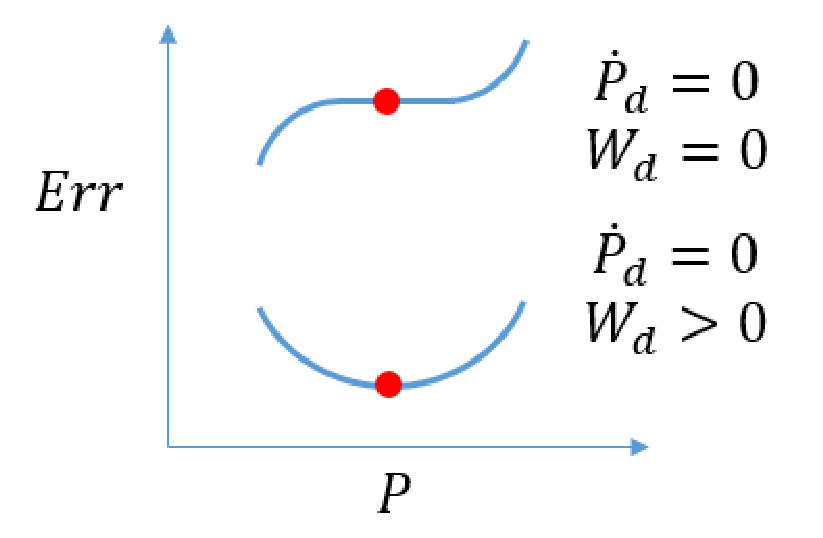
\includegraphics[width=1.8in]{error_graphs_modified}
    \caption{Top Line: moving the point does not change the error, thus the desired movement is zero, however, it is not important to achieve zero movement, thus $W_d = 0$.  Bottom Line: error is at a local minimum; thus moving the point increases error.}
    % \vspace{-0.2in}
    \label{fig:error_examples}
\end{figure}
% \end{minipage}
\begin{algorithm}[t]
    \caption{ErrorCorrection$(\deformconfig, \deformtarget)$}
    \begin{algorithmic}[1]
        \State $\deformvelocity_e \gets \boldsymbol 0_{\deformconfigspacesize \times 1}$, $\pseudoinverseweight_e \gets \boldsymbol 0_{\numdeformpoints \times 1}$
        \For{$i \in \{1,2,\dots,\numtargetpoints \}$}
            \State $k \gets \argmin_{j \in \{ 1,2,\dots,\numdeformpoints \}} \| \deformtarget_i - \deformconfig_j \|$
            \State $\deformvelocity_{e,k} \gets \deformvelocity_{e,k} + \deformtarget_i - \deformconfig_k$
            \State $\pseudoinverseweight_{e,k} \gets \max (\pseudoinverseweight_{e,k}, \| \deformtarget_i - \deformconfig_k \|)$
        \EndFor
        \State \Return $\{ \dot \deformconfig_e, \pseudoinverseweight_e \}$
    \end{algorithmic}
    \label{alg:error_correction}
\end{algorithm}
\begin{algorithm}[t]
    \caption{StretchingCorrection$(\relaxeddistancematrix, \lambda, \deformconfig)$}
    \begin{algorithmic}[1]
        \State $E \gets$ EuclidianDistanceMatrix$(\deformconfig)$
        \State $\deformvelocity_s \gets \boldsymbol 0_{3\numdeformpoints \times 1}$, $\pseudoinverseweight_s \gets \boldsymbol 0_{\numdeformpoints \times 1}$
        \State $\Delta \gets E - \relaxeddistancematrix$
        \For{$i \in \{1,2,\dots,\numdeformpoints \}$}
            \For{$j \in \{i+1,\dots,\numdeformpoints \}$}
                \If{$\Delta_{i,j} > \lambda$}
                    \State $v \gets \Delta_{i,j}(\deformconfig_j - \deformconfig_i)$
                    \State $\deformvelocity_{s,i} \gets \deformvelocity_{s,i} + \frac{1}{2}v$
                    \State $\deformvelocity_{s,j} \gets \deformvelocity_{s,j} - \frac{1}{2}v$
                    \State $\pseudoinverseweight_{s,i} \gets \max (\pseudoinverseweight_{s,i}, \Delta_{i,j})$
                    \State $\pseudoinverseweight_{s,j} \gets \max (\pseudoinverseweight_{s,j}, \Delta_{i,j})$
                \EndIf
            \EndFor
        \EndFor
        \State \Return $\{ \deformvelocity_s, \pseudoinverseweight_s \}$
    \end{algorithmic}
    \label{alg:stretching_correction}
\end{algorithm}
\begin{algorithm}[t]
    \caption{CombineTerms$(\deformvelocity_e, \pseudoinverseweight_e, \deformvelocity_s, \pseudoinverseweight_s)$}
    \begin{algorithmic}[1]
        \For{$i \in \{ 1,2,\dots,\numdeformpoints \}$}
            \State $\deformvelocity_{d,i} \gets \deformvelocity_{s,i} + \left( \deformvelocity_{e,i} - \proj_{\deformvelocity_{s,i}} \deformvelocity_{e,i} \right)$
            \State $\pseudoinverseweight_{d,i} \gets \pseudoinverseweight_{s,i} + \pseudoinverseweight_{e,i}$
        \EndFor
        \State \Return $\{ \deformvelocity_d, \pseudoinverseweight_d \}$
    \end{algorithmic}
    \label{alg:combine_terms}
\end{algorithm}
\begin{algorithm}[t]
    \caption{ObstacleRepulsion$(\obstacle, \beta)$}
    \begin{algorithmic}[1]
        \For{$\gripperindex \in \{1,2,\dots, \numgrippers\}$}
            \State $J_{p^g}, \dot x _{p^g}, d_g \gets$ Proximity$(\obstacle, \gripperindex)$
            \State $\gamma \gets e^{-\beta d_g}$
            \State $\robotvelocity_{c,g} \gets J_{p^g}^+ \dot x_{p^g}$
            \State $\robotvelocity_{c,g} \gets \frac{\maxgrippervelobstacle}{\| \robotvelocity_{c,g} \|} \robotvelocity_{c,g}$
            \State  $\robotvelocity_{\gripperindex} \gets \gamma \left( \robotvelocity_{c,g} + \left( \eye - J_{p^g}^+ J_{p^g} \right) \robotvelocity_\gripperindex \right) + (1-\gamma)\robotvelocity_\gripperindex$
        \EndFor        
        \State \Return $\robotvelocity$
    \end{algorithmic}
    \label{alg:obstaclerepulsion}
\end{algorithm}
\begin{algorithm}[t]
    \caption{Proximity$(\gripperindex, \obstacle)$ - reproduced from~\cite{Berenson2013}}
    \label{alg:proximity}
    \begin{algorithmic}[1]
        \State $d_\gripperindex \gets \infty$
        \For{$o \in \{1,2,\dots,|\obstacle|\}$}
            \State $p^\gripperindex, p^o \gets$ ClosestPoints$(\gripperindex, o)$
            \State $v \gets p^\gripperindex - p^o$
            \If{$\| v \| < d_\gripperindex$}
                \State $d_\gripperindex \gets \| v \|$
                \State $\dot x_{p^\gripperindex} \gets \frac{v}{\| v \|}$
                \State $J_{p^\gripperindex} \gets$ GripperPointJacobian$(\gripperindex, p^\gripperindex)$
            \EndIf
        \EndFor
        \State \Return $\{J_{p^\gripperindex}, x_{p^\gripperindex}, d_\gripperindex \}$
    \end{algorithmic}
\end{algorithm}

\subsubsection{Error Correction}

We build on previous work~\cite{Berenson2013}, splitting the desired deformable object movement into two parts: an error correction part and a stretching correction part. When defining the direction we want to move the deformable object to minimize error we calculate two values; which direction to move the deformable object points $\deformvelocity_e$ and the importance of moving each deformable object point $\pseudoinverseweight_e$. This is analogous to computing the gradient of error, as well as an ``importance factor'' for each part of the gradient. We need these weights to be able to differentiate between points of the object where the error function is a plateau versus points where the error function is at a local minimum~(Fig.~\ref{fig:error_examples}). Typically this is achieved using a Hessian, however our error function does not have a second derivative at many points. We use the \texttt{ErrorCorrection} (Alg.~\ref{alg:error_correction}) function to calculate these values. Each target point $\deformtarget_i \in \deformtarget$ defines a potential field, pulling the nearest point on the deformable object $\deformconfig_k$ towards $\deformtarget_i$. $\pseudoinverseweight_e$ is set to the maximum distance $\deformconfig_k$ is being pulled by any target point. This allows $\pseudoinverseweight_e$ to be insensitive to changes in discretization.

% \begin{wrapfigure}[21]{r}{0.5\textwidth}
% \begin{wrapfigure}[38]{r}{0.5\textwidth}
    % % \begin{minipage}{0.5\textwidth}
\begin{figure}[t]
    \centering
    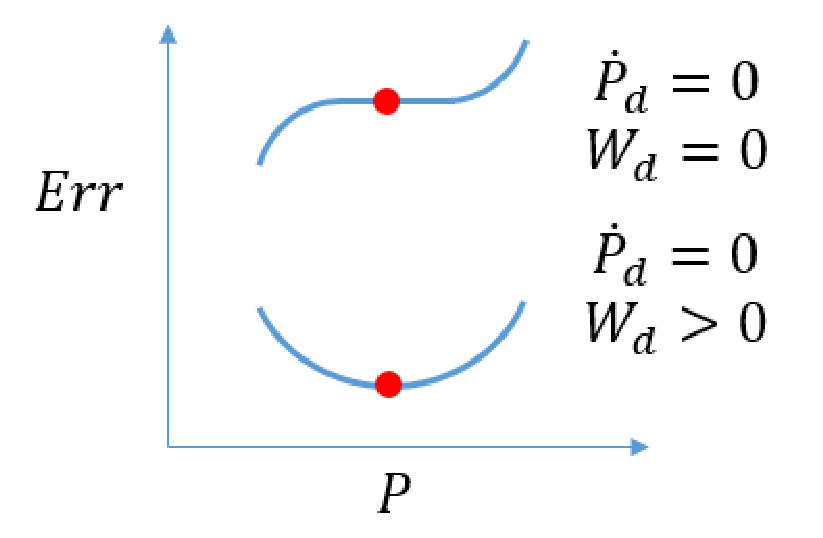
\includegraphics[width=1.8in]{error_graphs_modified}
    \caption{Top Line: moving the point does not change the error, thus the desired movement is zero, however, it is not important to achieve zero movement, thus $W_d = 0$.  Bottom Line: error is at a local minimum; thus moving the point increases error.}
    % \vspace{-0.2in}
    \label{fig:error_examples}
\end{figure}
% \end{minipage}
    % \vspace{-0.55in}
    % \begin{minipage}{0.5\textwidth}
        % \begin{algorithm}[t]
    \caption{ErrorCorrection$(\deformconfig, \deformtarget)$}
    \begin{algorithmic}[1]
        \State $\deformvelocity_e \gets \boldsymbol 0_{\deformconfigspacesize \times 1}$, $\pseudoinverseweight_e \gets \boldsymbol 0_{\numdeformpoints \times 1}$
        \For{$i \in \{1,2,\dots,\numtargetpoints \}$}
            \State $k \gets \argmin_{j \in \{ 1,2,\dots,\numdeformpoints \}} \| \deformtarget_i - \deformconfig_j \|$
            \State $\deformvelocity_{e,k} \gets \deformvelocity_{e,k} + \deformtarget_i - \deformconfig_k$
            \State $\pseudoinverseweight_{e,k} \gets \max (\pseudoinverseweight_{e,k}, \| \deformtarget_i - \deformconfig_k \|)$
        \EndFor
        \State \Return $\{ \dot \deformconfig_e, \pseudoinverseweight_e \}$
    \end{algorithmic}
    \label{alg:error_correction}
\end{algorithm}
        % \vspace{-0.57in}
        % \begin{algorithm}[t]
    \caption{StretchingCorrection$(\relaxeddistancematrix, \lambda, \deformconfig)$}
    \begin{algorithmic}[1]
        \State $E \gets$ EuclidianDistanceMatrix$(\deformconfig)$
        \State $\deformvelocity_s \gets \boldsymbol 0_{3\numdeformpoints \times 1}$, $\pseudoinverseweight_s \gets \boldsymbol 0_{\numdeformpoints \times 1}$
        \State $\Delta \gets E - \relaxeddistancematrix$
        \For{$i \in \{1,2,\dots,\numdeformpoints \}$}
            \For{$j \in \{i+1,\dots,\numdeformpoints \}$}
                \If{$\Delta_{i,j} > \lambda$}
                    \State $v \gets \Delta_{i,j}(\deformconfig_j - \deformconfig_i)$
                    \State $\deformvelocity_{s,i} \gets \deformvelocity_{s,i} + \frac{1}{2}v$
                    \State $\deformvelocity_{s,j} \gets \deformvelocity_{s,j} - \frac{1}{2}v$
                    \State $\pseudoinverseweight_{s,i} \gets \max (\pseudoinverseweight_{s,i}, \Delta_{i,j})$
                    \State $\pseudoinverseweight_{s,j} \gets \max (\pseudoinverseweight_{s,j}, \Delta_{i,j})$
                \EndIf
            \EndFor
        \EndFor
        \State \Return $\{ \deformvelocity_s, \pseudoinverseweight_s \}$
    \end{algorithmic}
    \label{alg:stretching_correction}
\end{algorithm}
    % \end{minipage}
    % \vspace{-0.62in}
% \end{wrapfigure}

\subsubsection{Stretching Correction}

Our algorithm for stretching correction is similar to that found in~\cite{Berenson2013}, with the addition of a weighting term $\pseudoinverseweight_s$, and a change in how we combine the two terms. We use the \texttt{StretchingCorrection} function (Alg.~\ref{alg:stretching_correction}) to compute $\deformvelocity_s$ and $\pseudoinverseweight_s$ based on a task-defined stretching threshold $\lambda \geq 0$. First we compute the distance between every two points on the object and store the result in $E$. We then compare $E$ to $D$ which contains the relaxed lengths between every pair of points. If any two points are stretched by more than $\lambda$, we attempt to move the points closer to each other. We use the same strategy for setting the importance of this stretching correction $\pseudoinverseweight_s$ as we use for error correction. When combining stretching correction and error correction terms (Alg.~\ref{alg:combine_terms}) we prioritize stretching correction, accepting only the portion of the error correction that is orthogonal to the stretching correction term for each point.

\subsubsection{Obstacle Avoidance}

% \begin{wrapfigure}{r}{0.5\textwidth}
    % \vspace{-0.55in}
    % \begin{minipage}{\columnwidth}
        % \vspace{-0.05in}
        % \begin{algorithm}[t]
    \caption{CombineTerms$(\deformvelocity_e, \pseudoinverseweight_e, \deformvelocity_s, \pseudoinverseweight_s)$}
    \begin{algorithmic}[1]
        \For{$i \in \{ 1,2,\dots,\numdeformpoints \}$}
            \State $\deformvelocity_{d,i} \gets \deformvelocity_{s,i} + \left( \deformvelocity_{e,i} - \proj_{\deformvelocity_{s,i}} \deformvelocity_{e,i} \right)$
            \State $\pseudoinverseweight_{d,i} \gets \pseudoinverseweight_{s,i} + \pseudoinverseweight_{e,i}$
        \EndFor
        \State \Return $\{ \deformvelocity_d, \pseudoinverseweight_d \}$
    \end{algorithmic}
    \label{alg:combine_terms}
\end{algorithm}
        % \vspace{-0.57in}
        % \begin{algorithm}[t]
    \caption{ObstacleRepulsion$(\obstacle, \beta)$}
    \begin{algorithmic}[1]
        \For{$\gripperindex \in \{1,2,\dots, \numgrippers\}$}
            \State $J_{p^g}, \dot x _{p^g}, d_g \gets$ Proximity$(\obstacle, \gripperindex)$
            \State $\gamma \gets e^{-\beta d_g}$
            \State $\robotvelocity_{c,g} \gets J_{p^g}^+ \dot x_{p^g}$
            \State $\robotvelocity_{c,g} \gets \frac{\maxgrippervelobstacle}{\| \robotvelocity_{c,g} \|} \robotvelocity_{c,g}$
            \State  $\robotvelocity_{\gripperindex} \gets \gamma \left( \robotvelocity_{c,g} + \left( \eye - J_{p^g}^+ J_{p^g} \right) \robotvelocity_\gripperindex \right) + (1-\gamma)\robotvelocity_\gripperindex$
        \EndFor        
        \State \Return $\robotvelocity$
    \end{algorithmic}
    \label{alg:obstaclerepulsion}
\end{algorithm}
        % \vspace{-0.57in}
        % \begin{algorithm}[t]
    \caption{Proximity$(\gripperindex, \obstacle)$ - reproduced from~\cite{Berenson2013}}
    \label{alg:proximity}
    \begin{algorithmic}[1]
        \State $d_\gripperindex \gets \infty$
        \For{$o \in \{1,2,\dots,|\obstacle|\}$}
            \State $p^\gripperindex, p^o \gets$ ClosestPoints$(\gripperindex, o)$
            \State $v \gets p^\gripperindex - p^o$
            \If{$\| v \| < d_\gripperindex$}
                \State $d_\gripperindex \gets \| v \|$
                \State $\dot x_{p^\gripperindex} \gets \frac{v}{\| v \|}$
                \State $J_{p^\gripperindex} \gets$ GripperPointJacobian$(\gripperindex, p^\gripperindex)$
            \EndIf
        \EndFor
        \State \Return $\{J_{p^\gripperindex}, x_{p^\gripperindex}, d_\gripperindex \}$
    \end{algorithmic}
\end{algorithm}
        % \vspace{-0.8in}
    % \end{minipage}
% \end{wrapfigure}
In order to guarantee that the grippers do not collide with any obstacles, we use the same strategy from~\cite{Berenson2013}, smoothly switching between collision avoidance and other objectives (see Alg.~\ref{alg:obstaclerepulsion}). For every gripper $\gripperindex$ and an obstacle set $\obstacle$ we find the distance $d_\gripperindex$ to the nearest obstacle, a unit vector $\dot x_{p_\gripperindex}$ pointing from the obstacle to the nearest point on the gripper, and a Jacobian $J_{p^\gripperindex}$ between the gripper's DOF and the point on the gripper as shown in Alg.~\ref{alg:proximity}. We then project the servoing motion from Eq.~\eqref{eqn:jacobianbackwardfunction} into the null space of the avoidance motion using the null space projector $\left(\eye - J_{p^g}^+ J_{p^g} \right)$. $\beta > 0$ sets the rate at which we change between servoing and collision avoidance objectives. $\maxgrippervelobstacle > 0$ is an internal parameter that sets how quickly we move the robot away from obstacles.

In principle the same null space avoidance can be used to prevent gripper-gripper collisions, but the tasks that we consider do not bring the the grippers close to each other in practice. Extensions to consider self collision and working with robot arms are discussed in Sec.~\ref{sec:real_robot}.
\subsection{Jacobian Models}
\label{sec:jacobian_models}

Every model must define a prediction function $\deformablemodelforwardfunction(\robotvelocity)$ and has an associated robot command function $\deformablemodelbackwardfunction(\deformvelocity, \pseudoinverseweight)$. This paper focuses on Jacobian-based models whose basic formulation Eq.~\eqref{eqn:jacobian} directly defines the deformation model $\deformablemodelforwardfunction$
\begin{equation}
    \deformablemodelforwardfunction(\robotvelocity) = J \robotvelocity \enspace.
    \label{eqn:jacobianforwardfunction}
\end{equation}
When defining the robot command function $\deformablemodelbackwardfunction$, we use the weights $\pseudoinverseweight$ to focus the robot motion on the important part of $\deformvelocity$. This is done by using a weighted norm in a standard minimization problem
% \begin{equation}
% \begin{aligned}
%     \deformablemodelbackwardfunction(\deformvelocity, \pseudoinverseweight) = 
%         &\argmin_{\robotvelocity }   & & \| J \robotvelocity - \deformvelocity \|^2_{\pseudoinverseweight} \\
%         & \text{subject to}          & & \| \robotvelocity \|^2 < \maxgrippervelservo^2
% \end{aligned}
% \end{equation}
\begin{equation}
    \begin{aligned}
        \deformablemodelbackwardfunction(\deformvelocity, \pseudoinverseweight) =
                    & \argmin_{\robotvelocity } 
                    & & \| J \robotvelocity - \deformvelocity \|^2_{\pseudoinverseweight} \\
                    &\text{subject to}           
                    & & \| \robotvelocity \|^2 < \maxgrippervelservo^2 \enspace.
        \label{eqn:jacobianbackwardfunction}
    \end{aligned}
\end{equation}
We also need to ensure that the grippers do not move too quickly, so we add the constraint that the robot moves no more than $\maxgrippervelservo > 0$. To solve \eqref{eqn:jacobianbackwardfunction} we use the Gurobi~\cite{Gurobi2016} optimizer. We use two different Jacobian approximation methods in our model set; a diminishing rigidity Jacobian, and an adaptive Jacobian, which are described below.


\subsubsection{Diminishing Rigidity Jacobian}

The key assumption used by this method~\cite{Berenson2013} is \textit{diminishing rigidity}: the closer a gripper is to a particular part of the deformable object, the more that part of the object moves in the same way that the gripper does (i.e. more ``rigidly''). The further away a given point on the object is, the less rigidly it behaves; the less it moves when the gripper moves. This approximation depends on two parameters $k_{trans} \geq 0$ and $k_{rot} \geq 0$ which control how the translational and rotational rigidity scales with distance. Small values entail very rigid objects; high values entail very deformable objects.

For every point $p_i \in \deformconfig$ and every gripper $\gripperindex$ we construct a Jacobian $J_{rigid}(q,i,g)$ such that if $p_i$ was rigidly attached to the gripper $g$ then
\begin{equation}
    \dot p_i = J_{\mathit{rigid}}(q,i,g) \dot \robotconfig_{\gripperindex} = 
    \begin{bmatrix}J_{trans}(q,i,g) & J_{rot}(q,i,g)\end{bmatrix}
    \dot \robotconfig_{\gripperindex} \enspace .
\end{equation}
Let $D_{i,g}$ be a measure of the distance between gripper $g$ and point $p_i$. Then the translational rigidity of point $p_i$ with respect to gripper $g$ is defined as
\begin{equation}
    w_{trans}(i,g) = e^{-k_{trans}D_{i,g}}
\end{equation}
and the rotational rigidity is defined as
\begin{equation}
    w_{rot}(i,g) = e^{-k_{rot}D_{i,g}}.
\end{equation}
To construct an approximate Jacobian $\tilde J(q)$ for a single point we combine the rigid Jacobians with their respective rigidity values
\begin{multline}
    \tilde J(q,i,g) = \\
    \begin{bmatrix}w_{trans}(i,g) J_{trans}(q,i,g) & w_{rot}(i,g) J_{rot}(q,i,g)\end{bmatrix} \enspace,
\end{multline}
and then combine the results into a single matrix
\begin{equation}
    \tilde J(q) = 
    \begin{bmatrix}
        \tilde J(q,1,1) & \tilde J(q,1,2) & \dots & \tilde J(q, 1, G) \\
        \tilde J(q,2,1) & \ddots \\
        \vdots \\
        \tilde J(q,P,1)
    \end{bmatrix} \enspace .
\end{equation}


\subsubsection{Adaptive Jacobian}

A different approach is taken in~\cite{Navarro-Alarcon2013}, instead using online estimation to approximate $J(q)$.
In this formulation we start with some estimate of the Jacobian $\tilde J(0)$ at time $t = 0$ and then use the Broyden update rule~\cite{Broyden1965} to update $\tilde J(t)$ at each timestep $t$
\begin{equation}
    \tilde J(t) = \tilde J(t-1) + \Gamma \frac{\left( \deformvelocity(t) - \tilde J(t-1) \robotvelocity(t) \right)}{\robotvelocity(t)^T \robotvelocity(t)} \robotvelocity(t)^T \enspace.
\end{equation}
This update rule depends on a update rate $\Gamma \in (0, 1]$ which controls how quickly the estimate shifts between timesteps.

